\newpage
\section{Работа развертки осциллографа}

При минимальном значении напряжения луч находится в крайнем левом положении на горизонтальной прямой экрана. По мере роста пилообразного напряжения луч перемещается слева направо с почти постоянной скоростью.

Луч за время прямого хода tпр переместится в крайнее правое положение экрана.  Когда напряжение спадает, луч совершает обратный ход — луч быстро возвращается в исходное положение, чтобы в следующий период повторить цикл, состоящий из прямого и обратного хода.

Чтобы линия развертки или изображение сигнала не мерцали при наблюдении, луч должен прочерчивать одну и ту же траекторию не менее 25-30 раз в секунду. 

При этом используется инерционная способность человеческого глаза сохранять зрительное впечатление примерно 1/15 с. Расчитанное для данного осциллографа время послесвечения ---- 1/43 с, т.е. для немерцающей траектории необходимо, чтобы луч вернулся в ранее пройденную точку не позже, чем через 1/43 секунды (частота 43 Гц).

\subsection{Осциллограмма сигнала}
\begin{figure}[H]
	\centering
	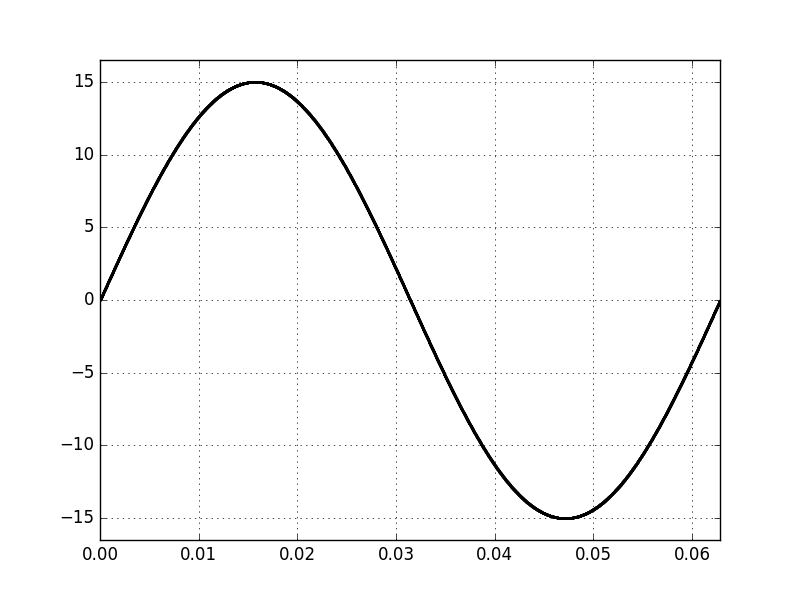
\includegraphics[width=0.85\textwidth]{freq-1-1.png}
	\caption{Осциллограмма сигнала для $\frac{m}{n}=\frac{1}{1}$}
	\label{fig:freq-1-1}
\end{figure}

\begin{figure}[H]
	\centering
	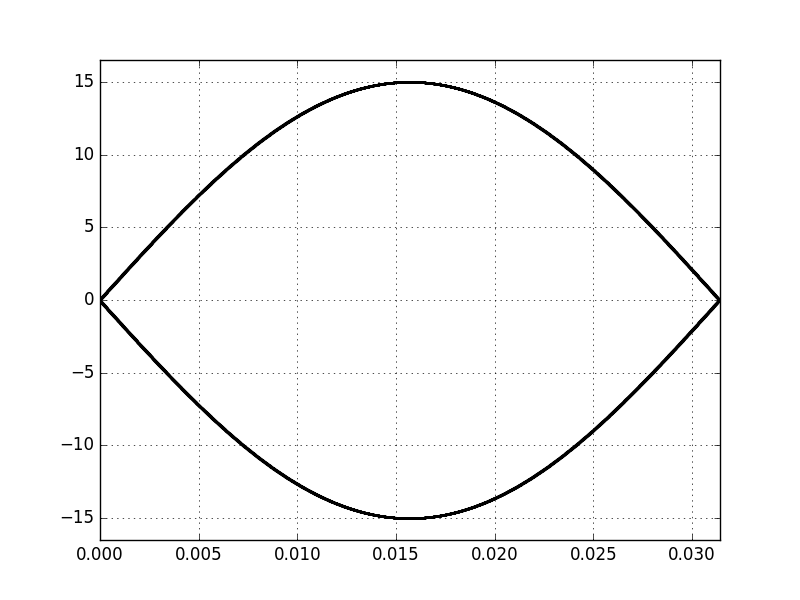
\includegraphics[width=0.85\textwidth]{freq-1-2.png}
	\caption{Осциллограмма сигнала для $\frac{m}{n}=\frac{1}{2}$}
	\label{fig:freq-1-2}
\end{figure}

\begin{figure}[H]
	\centering
	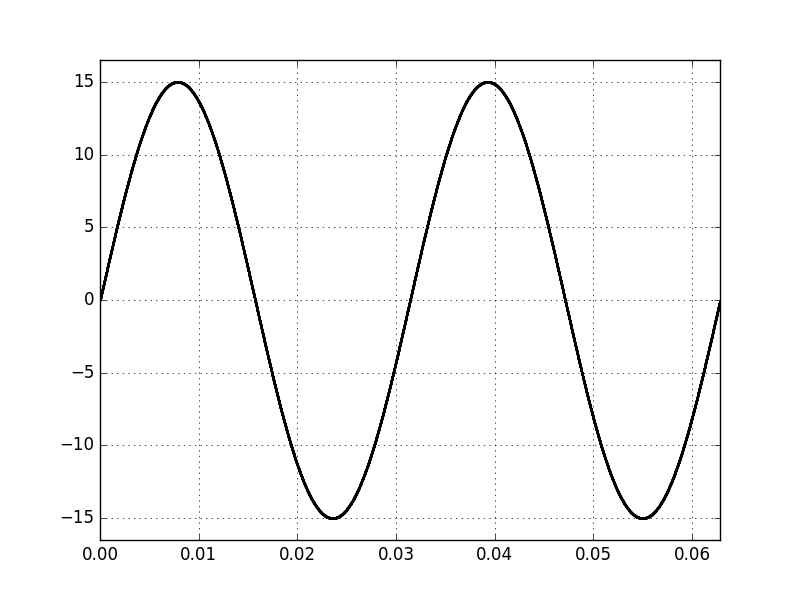
\includegraphics[width=0.85\textwidth]{freq-2-1.png}
	\caption{Осциллограмма сигнала для $\frac{m}{n}=\frac{2}{1}$}
	\label{fig:freq-2-1}
\end{figure}

\begin{figure}[H]
	\centering
	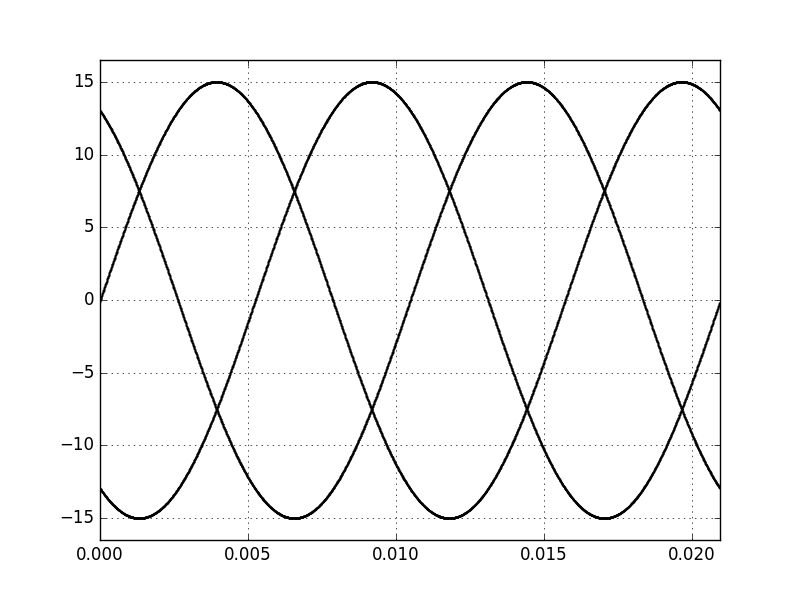
\includegraphics[width=0.85\textwidth]{freq-3-4.png}
	\caption{Осциллограмма сигнала для $\frac{m}{n}=\frac{3}{4}$}
	\label{fig:freq-3-4}
\end{figure}

\begin{figure}[H]
	\centering
	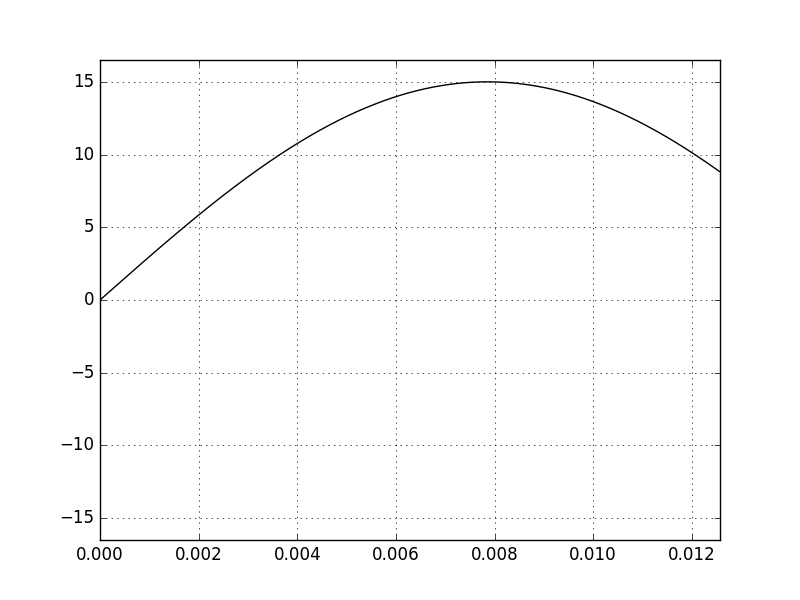
\includegraphics[width=0.85\textwidth]{freq-5-2.png}
	\caption{Осциллограмма сигнала для $\frac{m}{n}=\frac{5}{2}$}
	\label{fig:freq-5-2}
\end{figure}


\subsection{Бег осциллограммы}
\def\Tr{T_\text{р}}
\def\Ts{T_\text{с}}
При небольшой расстройке частот на осциллографе можно наблюдать движение (бег) несинхронизированной осциллограммы влево или вправо. 

Это явление легко иллюстрируется построением траектории движения луча по экрану в цикле развёртки. 

Если период развертки не равен периоду исследуемого сигнала, то график строится со сдвигом, причем если $\Tr<\Ts$, то сдвиг положительный (рис. \ref{fig:freq-1-0.95}).

В противном случае, если $\Tr>\Ts$, сдвиг то отрицательный  (рис. \ref{fig:freq-1-1.05}).

Отрисовка периодического сигнала со сдвигом создает иллюзию <<бега>> осциллограммы соответственно влево для отрицательного сдвига и вправо для положительного.

\begin{figure}[H]
	\centering
	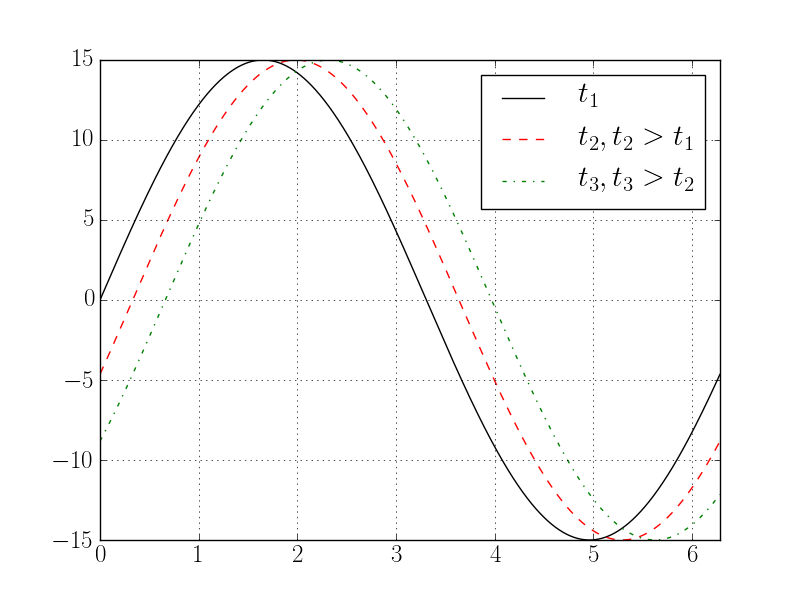
\includegraphics[width=0.85\textwidth]{freq-1-095.png}
	\caption{Бегущая развертка при $\frac{m}{n}=\frac{1}{0.95}$}
	\label{fig:freq-1-0.95}
\end{figure}
\begin{figure}[H]
	\centering
	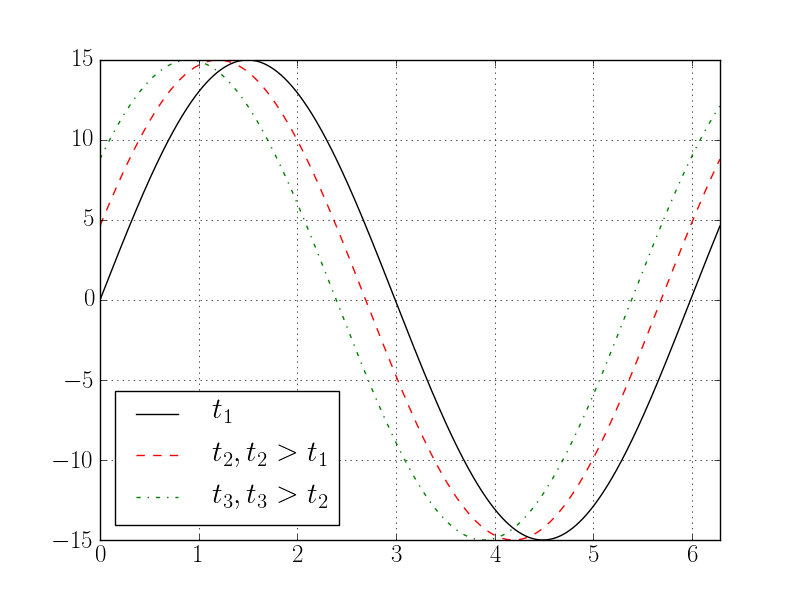
\includegraphics[width=0.85\textwidth]{freq-1-105.png}
	\caption{Бегущая развертка при $\frac{m}{n}=\frac{1}{1.05}$}
	\label{fig:freq-1-1.05}
\end{figure}
\subsection{Фигуры Лиссажу}
\begin{figure}[H]
	\centering
	% \hspace{-1cm}	
	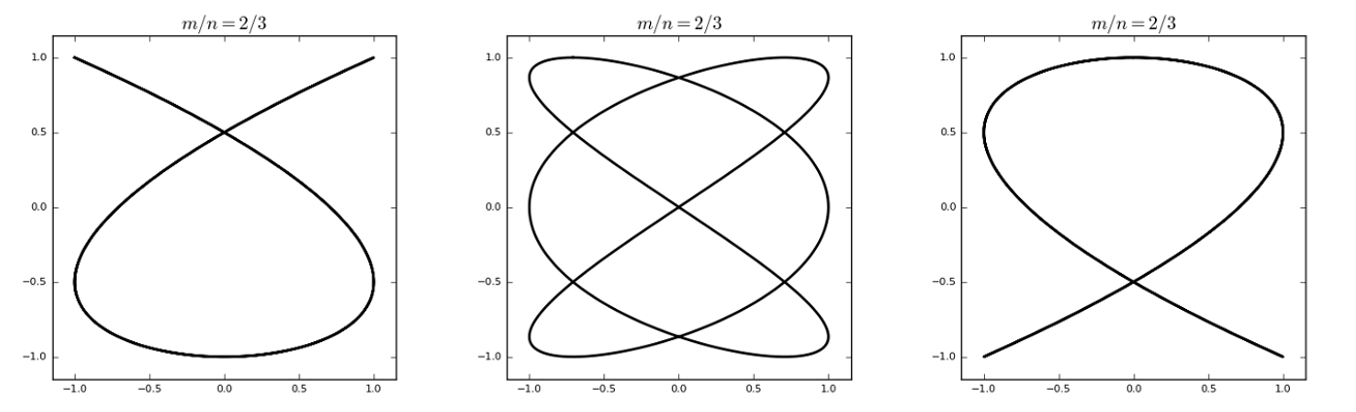
\includegraphics[width=0.85\textwidth]{lissajous2-3.png}
	\caption{Фигуры Лиссажу для $\frac{m}{n}=\frac{3}{2}$}
	\label{fig:lissajous-2}
\end{figure}
\begin{figure}[H]
	\centering
	% \hspace{-1cm}	
	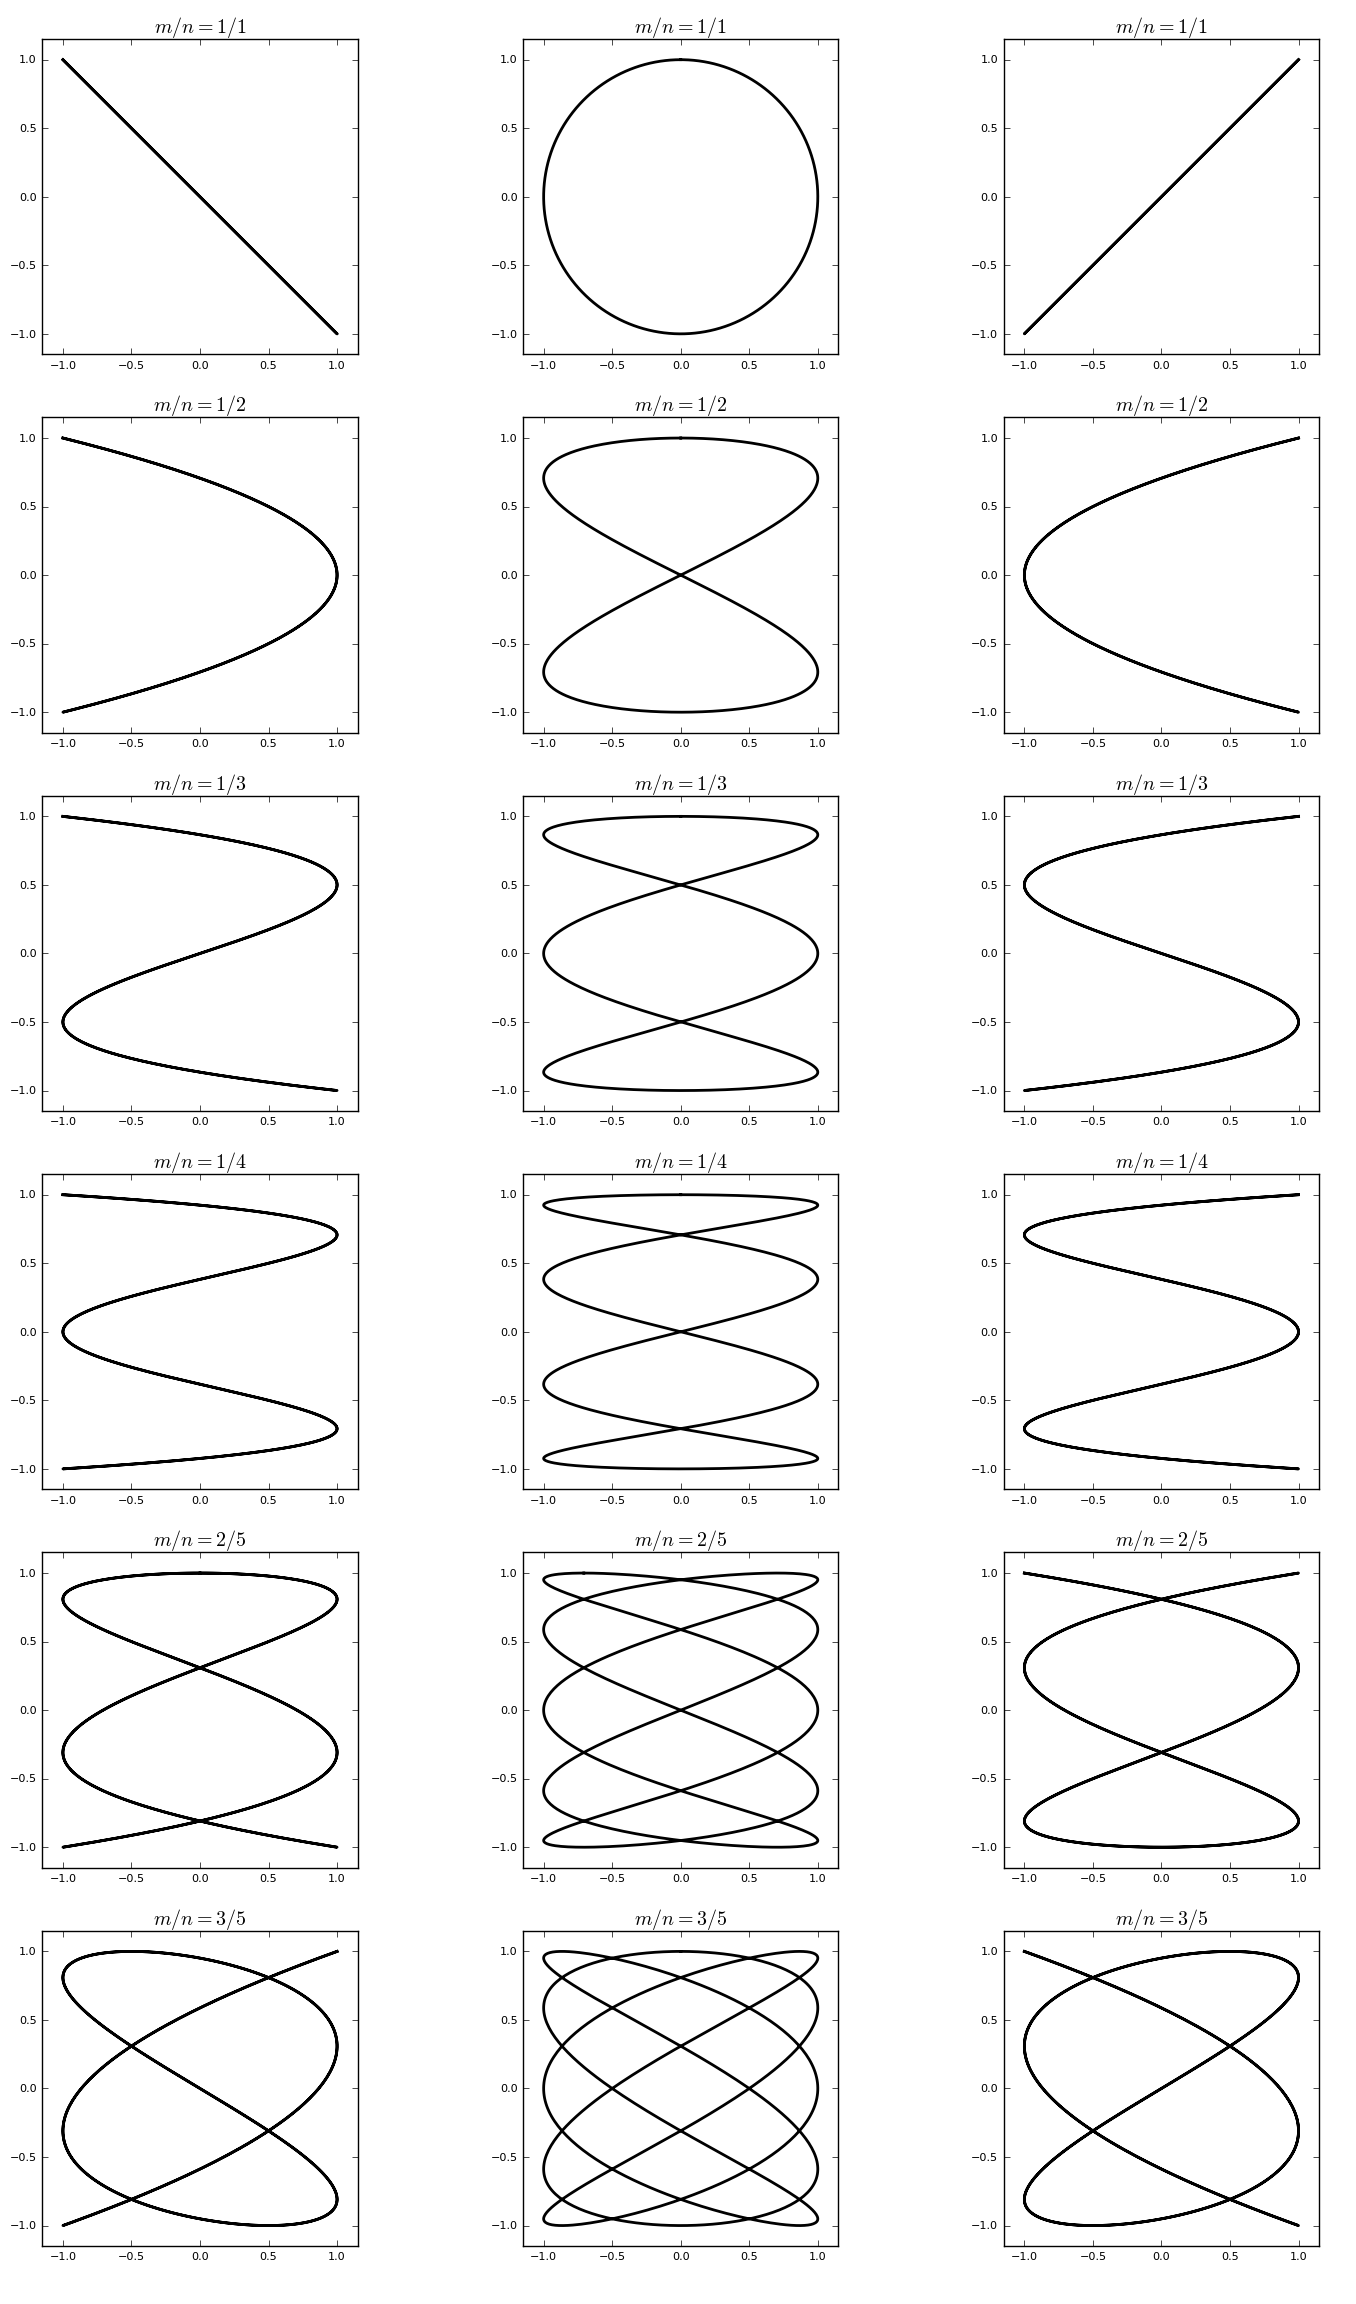
\includegraphics[width=0.8\textwidth]{lissajous3.png}
	\caption{Фигуры Лиссажу для $\frac{m}{n}=1;2;3;4;\frac{5}{2};\frac{5}{3}$}
	\label{fig:lissajous-1}
\end{figure}